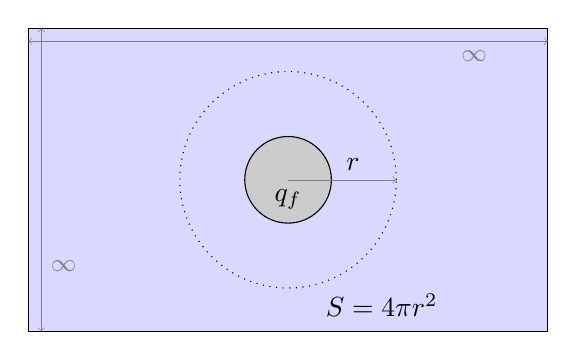
\begin{tikzpicture}[scale=1.1]
    \draw[fill=blue,fill opacity=0.15] (3,1.75) rectangle (-3,-1.75);

    \draw[fill=black!20!white] (0,0) circle (0.5); 
    \node[below] at (0,0) {$q_f$};

    \draw[dotted] (0,0) circle (1.25); 

    \draw[->,very thin,gray] (0,0)--(1.25,0);

    \node[above] at (0.75,0) {$r$};

    \node[below right] at (-75:1.25) {$S=4\pi r^2$};

    \draw[<->,gray,very thin] (-2.85,1.75)--(-2.85,-1.75);
    \draw[<->,gray,very thin] (-3,1.60)--(3,1.60);
    \node[right,gray] at (-2.85,-1.0) {\small $\infty$};
    \node[below,gray] at (2.15,1.60) {\small $\infty$};
\end{tikzpicture}
